\documentclass{article}

%% Created with wxMaxima 15.08.2

\setlength{\parskip}{\medskipamount}
\setlength{\parindent}{0pt}
\usepackage[utf8]{inputenc}
\DeclareUnicodeCharacter{00B5}{\ensuremath{\mu}}
\usepackage{graphicx}
\usepackage{color}
\usepackage{amsmath}
\usepackage{ifthen}
\newsavebox{\picturebox}
\newlength{\pictureboxwidth}
\newlength{\pictureboxheight}
\newcommand{\includeimage}[1]{
    \savebox{\picturebox}{\includegraphics{#1}}
    \settoheight{\pictureboxheight}{\usebox{\picturebox}}
    \settowidth{\pictureboxwidth}{\usebox{\picturebox}}
    \ifthenelse{\lengthtest{\pictureboxwidth > .95\linewidth}}
    {
        \includegraphics[width=.95\linewidth,height=.80\textheight,keepaspectratio]{#1}
    }
    {
        \ifthenelse{\lengthtest{\pictureboxheight>.80\textheight}}
        {
            \includegraphics[width=.95\linewidth,height=.80\textheight,keepaspectratio]{#1}
            
        }
        {
            \includegraphics{#1}
        }
    }
}
\DeclareMathOperator{\abs}{abs}
\usepackage{animate} % This package is required because the wxMaxima configuration option
                      % "Export animations to TeX" was enabled when this file was generated.

\definecolor{labelcolor}{RGB}{100,0,0}

\begin{document}

\noindent
%%%%%%%%%%%%%%%
%%% INPUT:
\begin{minipage}[t]{8ex}\color{red}\bf
\begin{verbatim}
-->  
\end{verbatim}
\end{minipage}
\begin{minipage}[t]{\textwidth}\color{blue}
\begin{verbatim}
Jaim271(x):= 
(((tanh((x-01)*20)+1)*(-tanh((x-05)*20)+1)/4)*(x-2)^2)+
(((tanh((x-06)*20)+1)*(-tanh((x-12)*20)+1)/4)*(-(x-9)^2+8))+
(((tanh((x-13)*20)+1)*(-tanh((x-13.5)*20)+1)/4)*8)+
(((tanh((x-15)*20)+1)*(-tanh((x-19)*20)+1)/4)*((x-17)^2+5))+
(((tanh((x-21)*20)+1)*(-tanh((x-27.1)*20)+1)/4)*2)+
(((tanh((x-21)*20)+1)*(-tanh((x-21.1)*20)+1)/4)*6)+
(((tanh((x-24)*20)+1)*(-tanh((x-24.1)*20)+1)/4)*3)+
(((tanh((x-27)*20)+1)*(-tanh((x-27.1)*20)+1)/4)*6);
\end{verbatim}
\end{minipage}
%%% OUTPUT:

\[\displaystyle
\parbox{10ex}{$\color{labelcolor}\mathrm{\tt (\%o150) }\quad $}
\mathrm{Jaim271}\left( x\right) :=\frac{\left( \mathrm{tanh}\left( \left( x-27\right) \cdot 20\right) +1\right) \cdot \left( 1-\mathrm{tanh}\left( \left( x-27.1\right) \cdot 20\right) \right) \cdot 6}{4}+\frac{\left( \mathrm{tanh}\left( \left( x-24\right) \cdot 20\right) +1\right) \cdot \left( 1-\mathrm{tanh}\left( \left( x-24.1\right) \cdot 20\right) \right) \cdot 3}{4}+\frac{\left( \mathrm{tanh}\left( \left( x-21\right) \cdot 20\right) +1\right) \cdot \left( 1-\mathrm{tanh}\left( \left( x-21.1\right) \cdot 20\right) \right) \cdot 6}{4}+\frac{\left( \mathrm{tanh}\left( \left( x-21\right) \cdot 20\right) +1\right) \cdot \left( 1-\mathrm{tanh}\left( \left( x-27.1\right) \cdot 20\right) \right) \cdot 2}{4}+\frac{\left( \mathrm{tanh}\left( \left( x-15\right) \cdot 20\right) +1\right) \cdot \left( 1-\mathrm{tanh}\left( \left( x-19\right) \cdot 20\right) \right) \cdot \left( {{\left( x-17\right) }^{2}}+5\right) }{4}+\frac{\left( \mathrm{tanh}\left( \left( x-13\right) \cdot 20\right) +1\right) \cdot \left( 1-\mathrm{tanh}\left( \left( x-13.5\right) \cdot 20\right) \right) \cdot 8}{4}+\frac{\left( \mathrm{tanh}\left( \left( x-6\right) \cdot 20\right) +1\right) \cdot \left( 1-\mathrm{tanh}\left( \left( x-12\right) \cdot 20\right) \right) \cdot \left( 8-{{\left( x-9\right) }^{2}}\right) }{4}+\frac{\left( \mathrm{tanh}\left( \left( x-1\right) \cdot 20\right) +1\right) \cdot \left( 1-\mathrm{tanh}\left( \left( x-5\right) \cdot 20\right) \right) \cdot {{\left( x-2\right) }^{2}}}{4}\mbox{}
\]
%%%%%%%%%%%%%%%


\noindent
%%%%%%%%%%%%%%%
%%% INPUT:
\begin{minipage}[t]{8ex}\color{red}\bf
\begin{verbatim}
-->  
\end{verbatim}
\end{minipage}
\begin{minipage}[t]{\textwidth}\color{blue}
\begin{verbatim}
wxplot2d(Jaim271(x), [x,-1,37], [y,-1,20] )$
\end{verbatim}
\end{minipage}
%%% OUTPUT:

\[\displaystyle
\parbox{10ex}{$\color{labelcolor}\mathrm{\tt (\%t151) }\quad $}
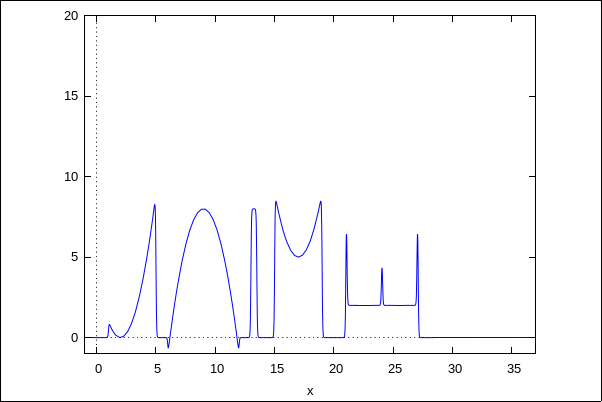
\includegraphics[width=.95\linewidth,height=.80\textheight,keepaspectratio]{Jaim2.71_img/Jaim2.71_1}\mbox{}
\]
%%%%%%%%%%%%%%%


\noindent
%%%%%%%%%%%%%%%
%%% INPUT:
\begin{minipage}[t]{8ex}\color{red}\bf
\begin{verbatim}
-->  
\end{verbatim}
\end{minipage}
\begin{minipage}[t]{\textwidth}\color{blue}
\begin{verbatim}
wxplot2d( [atan(x)/(%pi/2),tanh(x)], [x,-3,30], [y,-4,4] )$
\end{verbatim}
\end{minipage}
%%% OUTPUT:

\[\displaystyle
\parbox{10ex}{$\color{labelcolor}\mathrm{\tt (\%t133) }\quad $}
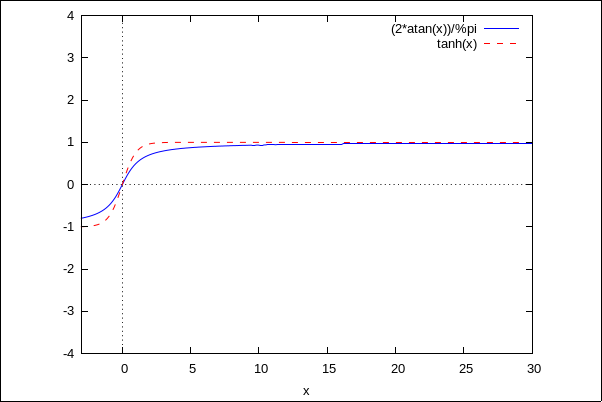
\includegraphics[width=.95\linewidth,height=.80\textheight,keepaspectratio]{Jaim2.71_img/Jaim2.71_2}\mbox{}
\]
%%%%%%%%%%%%%%%

\end{document}
